\documentclass[../main.tex]{subfiles}

\begin{document}
    El modelo termodinámico estima que la altura de hasta la cual se logra calentar la capa límite, debido al calor superficial es
    \begin{equation}
        H_t = \sqrt{ \frac{2 \int_0^{t} W dt}{ \left( \Gamma + \frac{g}{c_p} \right) \rho_0 c_p}   }  \label{Ht}
    \end{equation}
    con $W$ el flujo de calor superficial por unidad de tiempo $\left(\dfrac{\text{W}}{\text{m}^2} = \dfrac{\text{J}}{\text{s}\,\text{m}^2}\right)$.\\

En este modelo se supone que el perfil de temperatura inicial tiene un gradiente constante $\Gamma$, y que la capa se calienta de a poco de forma adiabática, tomando la pendiente $-\frac{g}{c_p}$

En la ecuación \eqref{Ht}, el término $\int_0^{t} W dt$ corresponde al área bajo la curva de flujo de calor sensible superficial. Esta la estimamos de la siguiente manera.

\begin{minipage}{\linewidth}
    \centering
    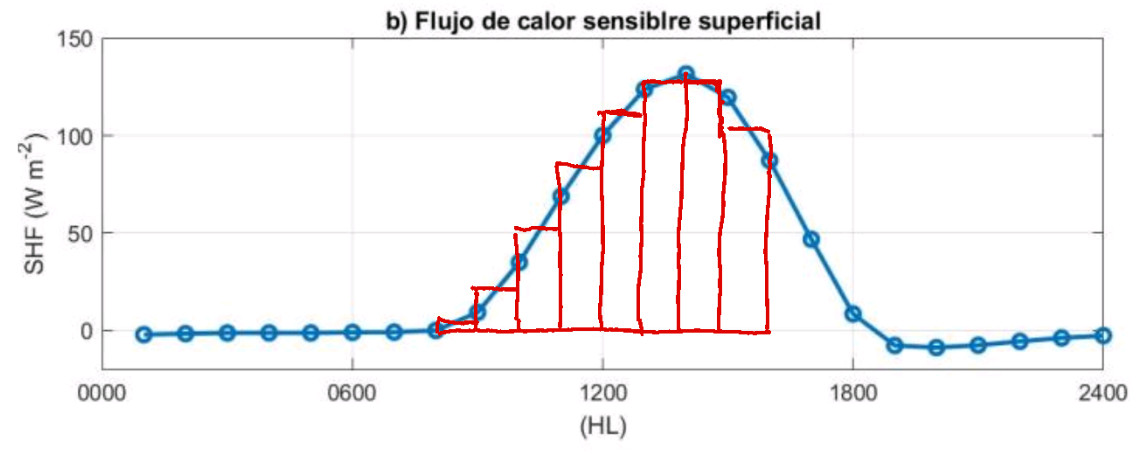
\includegraphics[width=0.8\textwidth]{img/area_WT}
    \captionof{figure}{Flujo de calor sensible superficial. Los bloques en rojo esquematizan la estimación del area bajo la curva en el rango solicitado (desde las 0800 hasta las 1600). Cada bloque tiene un ancho de 1 hora y la altura corresponde al promedio de los dos valores contiguos de SHF. }
    \label{aWT}
\end{minipage}\\

De manera visual, comparando con los valores de W (SHF) de los ``ticks'' del eje vertical, estimo que el área es aproximadamente 
\begin{equation}
    \int_0^{16} W(t)\, dt = 615 \frac{\text{Watt}}{\text{m}^2}\cdot \text{Hora} = 2214000 \dfrac{\text{J}}{\text{m}^2}.
\end{equation}


\end{document}
